%%%%%%%%%%%%%%%%%%%%%%%%%%%%%%%%%%%%%%%%%
% Short Sectioned Assignment
% LaTeX Template
% Version 1.0 (5/5/12)
%
% This template has been downloaded from:
% http://www.LaTeXTemplates.com
%
% Original author:
% Frits Wenneker (http://www.howtotex.com)
%
% License:
% CC BY-NC-SA 3.0 (http://creativecommons.org/licenses/by-nc-sa/3.0/)
%
%%%%%%%%%%%%%%%%%%%%%%%%%%%%%%%%%%%%%%%%%

%----------------------------------------------------------------------------------------
%	PACKAGES AND OTHER DOCUMENT CONFIGURATIONS
%----------------------------------------------------------------------------------------

\documentclass[paper=a4,fontsize=12pt]{scrartcl}

\usepackage[T1]{fontenc} % Use 8-bit encoding that has 256 glyphs
\usepackage[english]{babel} % English language/hyphenation
\usepackage{amsmath,amsfonts,amsthm,setspace} % Math packages
\usepackage{graphicx}
\usepackage[a4paper, total={7in, 10in}]{geometry}
\usepackage{multicol}
\usepackage{listings} 
\usepackage{beramono}
\usepackage{times}
\usepackage{hyperref}
%\usepackage{subcaption}
\usepackage{subfig}
\usepackage[format=plain]{caption}
\usepackage{placeins}
\usepackage{cleveref}

\graphicspath{{../CliffordReport/}{../HarrisonMethod/}}

\newcommand{\subfigureautorefname}{\figureautorefname}
\renewcommand{\autoref}[1]{\cref{#1}}

\allowdisplaybreaks

\lstset{tabsize=2,language=C++,basicstyle=\footnotesize\ttfamily}

%\usepackage{sectsty} % Allows customizing section commands
%\allsectionsfont{\centering \normalfont\scshape} % Make all sections centered, the default font and small caps

%\usepackage{fancyhdr} % Custom headers and footers
%\pagestyle{fancyplain} % Makes all pages in the document conform to the custom headers and footers
%\fancyhead{} % No page header - if you want one, create it in the same way as the footers below
%\fancyfoot[L]{} % Empty left footer
%\fancyfoot[C]{} % Empty center footer
%\fancyfoot[R]{\thepage} % Page numbering for right footer
%\renewcommand{\headrulewidth}{0pt} % Remove header underlines
%\renewcommand{\footrulewidth}{0pt} % Remove footer underlines
%\setlength{\headheight}{13.6pt} % Customize the height of the header

\numberwithin{equation}{section} % Number equations within sections (i.e. 1.1, 1.2, 2.1, 2.2 instead of 1, 2, 3, 4)
\numberwithin{figure}{section} % Number figures within sections (i.e. 1.1, 1.2, 2.1, 2.2 instead of 1, 2, 3, 4)
\numberwithin{table}{section} % Number tables within sections (i.e. 1.1, 1.2, 2.1, 2.2 instead of 1, 2, 3, 4)

%\setlength\parindent{0pt} % Removes all indentation from paragraphs - comment this line for an assignment with lots of text

%\renewcommand{\thesubsection}{\thesection.\alph{subsection}}

%----------------------------------------------------------------------------------------
%	TITLE SECTION
%----------------------------------------------------------------------------------------

\newcommand{\horrule}[1]{\rule{\linewidth}{#1}} % Create horizontal rule command with 1 argument of height

\title{	
\normalfont \normalsize 
\textsc{University of Western Ontario} \\ [25pt] % Your university, school and/or department name(s)
\horrule{0.5pt} \\[0.4cm] % Thin top horizontal rule
\Large CS9869b Course project\\ \huge Factorial analysis of fMRI data  \\ % The assignment title
\horrule{2pt} \\[0.5cm] % Thick bottom horizontal rule
}

\author{Dmitrii Marin \\ \small\tt dmarin3@uwo.ca} % Your name

\date{\normalsize\today} % Today's date or a custom date

\begin{document}

\maketitle % Print the title

\begin{abstract}

Functional magnetic resonance imaging (fMRI) is a procedure that uses MRI in order to measure brain activity via detecting changes in the blood flow in the brain. It has been shown that when a particular area in the brain is in use, blood flow to this area increases\cite{ogawa1990brain,shmuel2002sustained}. Known relation between the neuron activity and blood flow (the hemodynamic function) and regression analysis allow to relate measured fMRI time series with hypothesized stimuli or activity induced processes\cite{huettel2004functional}.  %The regression coefficients are time independent and indicate the relation between a brain voxel and the studied stimuli or activities. 
This allows to find a particular region of the brain responsible for studied activity or stimuli. Recently researches addressed a problem of interaction between different stimuli or activity. This is known as \emph{multiple factor analysis}.

This project addresses the problem of two factor analysis of fMRI data. In particular we are interesting in the following questions. Does a part of the brain (represented as a set of voxels) encode information about each of the factors independently or  resemble unique combination of factor levels. Kornysheva and Diedrichsen in \cite{Kornysheva2014} identified brain regions that are responsible for spatial or temporal features of finger move sequences. They also identified regions that had activation patterns decoding unique combinations of the features. They used classification approach. This project aims to explore and compare different approaches to this problem. We study classical \emph{multivariate analysis of variation} (manova) and also its cross-validate extension. We also explore \emph{Pattern Component Modeling}\cite{Walther2016}, which is based on \emph{Representational Similarity Analysis}~\cite{kriegeskorte2008representational}. We compare all three methods.


\end{abstract}

\newpage

\section*{Co-authorship statement}
Yuanhao Lai wrote \cref{sec:manova}. Harrison Ritz wrote \cref{sec:pcm}. 

\section*{Introduction}

 Kornysheva and Diedrichsen in \cite{Kornysheva2014} taught volunteers to perform series of finger movements. Each sequence was a combination of three different temporal (temporal factor) and three different spatial (spatial factor) features. They found the regions in the brain that encode each of the factors independently as well as the regions that encode unique features of all possible combinations in the brain. 

They used search light technique to mark the brain map. Whole set of voxels were divided into overlapping densely placed groups of 160 voxels. The factorial analysis was performed on each of the groups independently. To study different methods for factorial analysis we decided to conduct simulation experiments. We assume that our activation patterns $Y$ comes from the following model
\begin{equation}\tag{*}
\underset{\left(n\times p\right)}{Y}=\underset{\left(n\times k\right)}{Z}\underset{\left(k\times p\right)}{U}+\underset{\left(n\times p\right)}{E}
\label{eq:sim}
\end{equation}
where $Y$ is activation patterns of size 9x160 (9 combinations of factors for 160 voxels), $Z$ is a design matrix of size 9x15 (for each of 9 combinations defines that effects are present, there are 6 main effects and 9 interaction patterns), $U$ is a matrix of size 15x160 that shows the \emph{signal-to-noise-ratio} (SNR) for each of the effects at each voxel, $E$ is i.i.d. noise. 

In our experiments we fix the noise covariance matrix $cov(E)=I$. In our design equation \eqref{eq:sim} we generate each element of $U$ matrix as i.i.d normal noise. Within a row the standard deviation is fixed to a desired SNR of the corresponding effect (main or interaction). We assume that there are 6 independent runs of the experiment. This yields an activation matrix of size 54x160, which for simplicity we will refer to as $Y$.

The rest of the paper is organized as follows. \Cref{sec:manova} describes classical MANOVA approach and also discusses its cross-validation extension. \Cref{sec:classification} describes the original classification approach. \Cref{sec:pcm} describes a recent pattern component modeling approach. \Cref{sec:manova,sec:classification,sec:pcm} also provide the result of our simulation tests. \Cref{sec:discussion} summarizes the results.

\section{MANOVA and CVMANOVA}
\label{sec:manova}

\subsection{Model Structure}

The method, multivariate analysis of variance (MANOVA)\cite{fox2013hypothesis},
assumes our data are generated from the multivariate general linear
model (MGLM), 
\[
\underset{\left(n\times p\right)}{\boldsymbol{Y}}=\underset{\left(n\times k\right)}{\boldsymbol{Z}}\underset{\left(k\times p\right)}{\boldsymbol{U}}+\underset{\left(n\times p\right)}{\boldsymbol{E}}
\]
where $\boldsymbol{Y}$ specifies the signal at $n$ different time
points in $p$ voxels, $\boldsymbol{Z}$ is the design matrix with
$K$ conditions such as the constant, linear predictors, dummy variables
for categorical predictors, $\boldsymbol{U}$ is a matrix of regression
coefficients and $\boldsymbol{E}$ is a matrix of random errors. It
is assumed that $Z$ is of full column-rank $k$ and each of the $n$
rows of $E$ is an independent sample from a $p$-dimensional normal
distribution $\text{N}(\boldsymbol{0},\Sigma_{\epsilon})$. $\Sigma_{\epsilon}$
is the spatial covariance structure of the data. Notice that $n=m\times k$,
where $m$ is the number of runs.

The maximum likelihood estimator (MLE) for $\boldsymbol{U}$ is, 
\[
\hat{\boldsymbol{U}}=\left(\boldsymbol{Z}^{T}\boldsymbol{Z}\right)^{-1}\boldsymbol{Z}^{T}\boldsymbol{Y}
\]



\subsection{Hypothesis Test}

We are interested in testing if there is any difference between patterns.
The null hypothesis is set as, 
\[
H_{0}:\ \underset{\left(q\times k\right)}{\boldsymbol{C}^{T}}\underset{\left(k\times p\right)}{\boldsymbol{U}}=\boldsymbol{0}
\]
where $\boldsymbol{C}$ is a $k\times q$ a contrast matrix of the
parameters, with rank $q\le k$.


\subsection{MANOVA\label{sub:MANOVA}}

To construct a test statistic, we first define the following two important
components, which are similar to the uni-variate case.

The regression sum of square, 
\begin{equation}
\boldsymbol{Q}_{h}=\hat{\boldsymbol{U}}^{T}\boldsymbol{H}^{T}\boldsymbol{Z}^{T}\boldsymbol{Z}\boldsymbol{H}\hat{\boldsymbol{U}}\label{eq:MANOVAQh}
\end{equation}
where $\boldsymbol{H}=\boldsymbol{C}\left(\boldsymbol{C}^{T}\boldsymbol{C}\right)^{-1}\boldsymbol{C}^{T}$
is the hypothesis matrix corresponding to the contrast $\boldsymbol{C}$.

The residual sum of square,
\begin{equation}
\boldsymbol{Q}_{e}=\left(\boldsymbol{Y}-\boldsymbol{Z}\hat{\boldsymbol{U}}\right)^{T}\left(\boldsymbol{Y}-\boldsymbol{Z}\hat{\boldsymbol{U}}\right)\label{eq:MANOVAQe}
\end{equation}
which is also an estimator for the (spatial) covariance structure
$\Sigma_{\epsilon}$ of the data, as $\hat{\Sigma}_{\epsilon}=\frac{1}{n}\boldsymbol{Q}_{e}$.

Using $\boldsymbol{Q}_{h}$ and $\boldsymbol{Q}_{e}$, we can construct
three types of test statistics for MANOVA, namely, the Wilks' lambda,
the Pillai's trace and the Barlett-Lawley-Hottellings trace. Those
statistics are different in the power in different situations. Normally,
Wilks' lambda is used as it is a likelihood ratio test statistic and
it is ensured to be the uniformly most powerful test though not the
most powerful test in a certain case. Wilks' lambda is defined as
below,

\begin{equation}
\Lambda=\frac{\det\left(\boldsymbol{Q}_{e}\right)}{\det\left(\boldsymbol{Q}_{h}+\boldsymbol{Q}_{e}\right)}=\prod_{i}\frac{1}{1+\lambda_{i}}
\end{equation}
where $\lambda_{i}$ are the solutions of the characteristic equation
$\mid\boldsymbol{Q}_{h}-\lambda\boldsymbol{Q}_{e}\mid=0$.

In addition, the $F$ approximation \cite{rao1951asymptotic} to the
null distribution of Wilks's Lambda is available, 
\[
F=\left[\Lambda^{\frac{-1}{t_{3}}}-1\right]\cdot\frac{\text{df}_{2}}{\text{df}_{1}}\sim F_{\text{df}_{1},\text{df}_{2}}
\]
where $t_{1}=n-k-\frac{p-q+1}{2}$, $t_{2}=\frac{pq-2}{4}$, $t_{3}=\begin{cases}
\sqrt{\frac{\left(pq\right)^{2}-4}{p^{2}+q^{2}-5}}, & p^{2}+q^{2}-5>0\\
1, & p^{2}+q^{2}-5\le0
\end{cases}$, $\text{df}_{1}=pq$ and $\text{df}_{2}=t_{1}\cdot t_{3}-2t_{2}$. 

\textbf{Notice} that the approximated $F$ distribution fails when
$n-k\ge p$ because $\text{df}_{2}$ may be less than $0$. The essential
reason is that $\boldsymbol{Q}_{e}$ defined by eqn.(\ref{eq:MANOVAQe})
is not positive-definite in this case and hence the computation of
the statistic is not feasible. To overcome this problem, we proposed
using the principle component analysis to reduce the number of voxels.
We would discuss it later in the Result section. 


\subsection{CV-MANOVA}

In the case where we want to quantify the distinctness between patterns,
we prefer the Barlett-Lawley-Hottellings trace because its equivalent
relationship to the Mahalanobis distance as shown by Allefeld \cite{allefeld2014searchlight}.
However, the Barlett-Lawley-Hottellings trace is severely biased,
so Allefeld used the cross-validated version of the Barlett-Lawley-Hottellings
trace to make it unbiased. The idea is very simple. He replaced the
estimated pattern $\hat{U}$ in eqn.(\ref{eq:MANOVAQh}) with its
cross-validated version. This alternative approach under the same
MGLM framework is called the cross-validated MANOVA (CV-MANOVA). The
resulted statistic by the \textquoteleft leave-one-run-out\textquoteright{}
cross-validation is,

\begin{equation}
D=\frac{(m-1)\left(n-k\right)-p-1}{(m-1)n}\cdot\frac{1}{m}\sum_{l=1}^{m}\sum_{h\neq l}\text{trace}\left[\boldsymbol{Q}_{h}^{CV}\left(\boldsymbol{Q}_{e}\right)^{-1}\right]\label{eq:CVMANOVA}
\end{equation}
where $\boldsymbol{Q}_{h}^{CV}=\hat{\boldsymbol{U}}^{(h)T}\boldsymbol{H}^{T}\boldsymbol{Z}^{(l)T}\boldsymbol{Z}^{(l)}\boldsymbol{H}\hat{\boldsymbol{U}}^{(l)}$
and $\hat{\boldsymbol{U}}^{(h)}$ is the MLE of $\boldsymbol{\boldsymbol{U}}$
using only the $h$th run data. However, CV-MANOVA suffered the same
problem as MANOVA for $\boldsymbol{Q}_{e}$ when $n-k\ge p$. But
since our simulated data is assumed to be (spatially) prewhitened
, $\boldsymbol{Q}_{e}=\hat{\Sigma}_{\epsilon}$ can be estimated as
a diagonal matrix where the diagonal elements are the same as eqn.(\ref{eq:MANOVAQe}).
However, there is not an exact distribution or a good approximated
distribution for this statistic. So the distribution under $H_{0}$
of the CV-MANOVA is obtained by either simulations or permutations. 


\subsection{Relationship between CV-MANOVA and RSA}

It can be shown the CV-MANOVA $D$ is also a linear contrasts of the
second moment matrix $\hat{G}$. If we ignored a constant scale of
the cross-validated Barlett-Lawley-Hottellings trace in eqn.(\ref{eq:CVMANOVA}),
then

\begin{eqnarray*}
D & = & \sum_{l=1}^{m}\sum_{h\neq l}\text{trace}\left[\boldsymbol{Q}_{h}^{CV}\left(\boldsymbol{Q}_{e}\right)^{-1}\right]\\
 & = & \sum_{l=1}^{m}\sum_{h\neq l}\text{trace}\left[\hat{\boldsymbol{U}}^{(h)T}\boldsymbol{H}^{T}\boldsymbol{Z}^{(l)T}\boldsymbol{Z}^{(l)}\boldsymbol{H}\hat{\boldsymbol{U}}^{(l)}\left(\hat{\Sigma}_{\epsilon}\right)^{-1}\right]\\
 & = & \sum_{l=1}^{m}\sum_{h\neq l}\text{trace}\left[\hat{\boldsymbol{U}}^{(h)T}\boldsymbol{H}^{T}\boldsymbol{Z}^{(l)T}\boldsymbol{Z}^{(l)}\boldsymbol{H}\hat{\boldsymbol{U}}^{(l)}\left(\hat{\Sigma}_{\epsilon}\right)^{-1}\hat{\boldsymbol{U}}^{(h)T}\right],\ \text{by the property of matrix trace}\\
 & = & (m-1)m\times\text{trace}\left[\boldsymbol{H}^{T}\boldsymbol{Z}^{(l)T}\boldsymbol{Z}^{(l)}\boldsymbol{H}\hat{G}\right]\\
 & \Rightarrow & \text{trace}\left[\boldsymbol{H}^{T}\boldsymbol{H}\hat{G}\right],\ \text{if the design is balanced,}\boldsymbol{Z}^{(l)T}\boldsymbol{Z}^{(l)}\approx cI\\
 & = & \text{trace}\left[\boldsymbol{H}\hat{G}\right],\ \boldsymbol{H}\text{ is idempotent and symmetric}\\
 & = & \sum_{i,j}\boldsymbol{H}_{ij}\hat{G}_{ij}
\end{eqnarray*}
Both CV-MANOVA and RSA estimate $\hat{\boldsymbol{U}}$ for all terms
simultaneously, so they have the same $\hat{G}$. Therefore, the equivalence
between CV-MANOVA and RSA require using the same hypothesis matrix
$\boldsymbol{H}$ and $Z^{T}Z\approx cI$ , where $c$ is a constant.
However, $\boldsymbol{H}$ is not necessarily the same for CV-MANOVA
and RSA. Although $\boldsymbol{H}$ for both methods are based on
the same contrast matrix, the construction procedures from the contrast
matrix to $\boldsymbol{H}$ are different. For example, if we are
interested in testing if any of the main effects, the interaction
and the overall (intercept) effect are significant, then we will have
four contrast matrices $C_{\text{main 1}}$, $C_{\text{main 2}}$,
$C_{\text{interaction}}$ and $C_{\text{intercept}}$ and we will
need four hypothesis matrices based on them. But CV-MANOVA forms four
$\boldsymbol{H}$'s independently each contrast matrix, while RSA
forms four $\boldsymbol{H}$'s from the combinations of all contrast
matrices. If we are only interested in testing $C_{\text{main 1}}$
and $C_{\text{main 2}}$, then $\boldsymbol{H}$'s formed by the CV-MANOVA
and RSA will be the same because the $C_{\text{main 1}}$ and $C_{\text{main 2}}$
are linearly independent, but this is not true when $C_{\text{interaction}}$
is involved. From this point of view, we may prefer RSA though they
should have similar performances.


\subsection{Results}

For all the statistical tests we performed, we specified type I error
i as 0.05. So the critical value for each method was obtained as the
95th percentile of the simulated/permuted distribution (one-sided
test).


\subsection{Limitation of MANOVA}

As we mentioned in Section \ref{sub:MANOVA}, MANOVA fails when $n-k\ge p$.
To overcome this problem, we introduced two simple methods and used
simulations to evaluate them . For the first method, we only utilized
the first 45 voxels and drop the remaining voxels. Figure \ref{fig:MANOVA1}
shows that the F approximation could still control the false positive
rate while retaining some powers. But this method was deficient as
it discarded a large amount of the original signals. A better approach
was to use the principal component analysis to reduce the dimensions
of voxels. Figure \ref{fig:CV-MANOVA-PCA} shows that for the number
of components between 25 to 30, the F approximation also controls
the false positive rate and achieves a much higher power. Figure \ref{fig:Explained-Variance-of}
also shows that the explained variances by these components are around
$70\%$.

\begin{figure}[H]
\begin{centering}
\subfloat{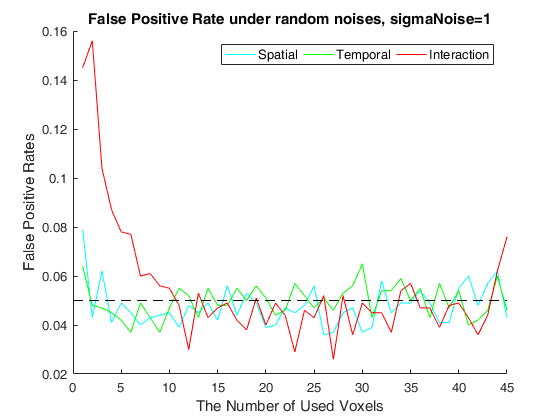
\includegraphics[scale=0.55]{0C__Users_Hao_Dropbox_NewtermPHD_TERM2_SS9833B_Analysis_of_brain_imaging_data_Report_MANOVA_Sig.png}}\subfloat{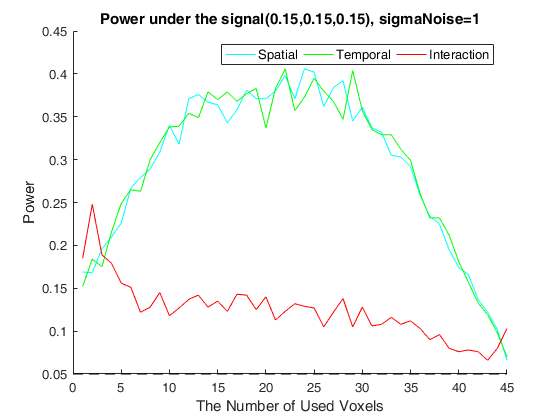
\includegraphics[scale=0.55]{1C__Users_Hao_Dropbox_NewtermPHD_TERM2_SS9833B____s_of_brain_imaging_data_Report_MANOVA_Power.png}}
\par\end{centering}

\centering{}\protect\caption{{\footnotesize{}MANOVA Using the first $N$ voxels ($N=1,\ldots,45$):
The left figure shows the false positive rates for detecting each
term from 1000 simulations of random noises. The right figure shows
the power for detecting each term from 1000 simulations of signals,
with 0.15 scale for each term. Under both cases, the variance for
the random error term is 1.}\label{fig:MANOVA1} }
\end{figure}


\begin{figure}[H]
\centering{}(0 indicates there is ).\subfloat{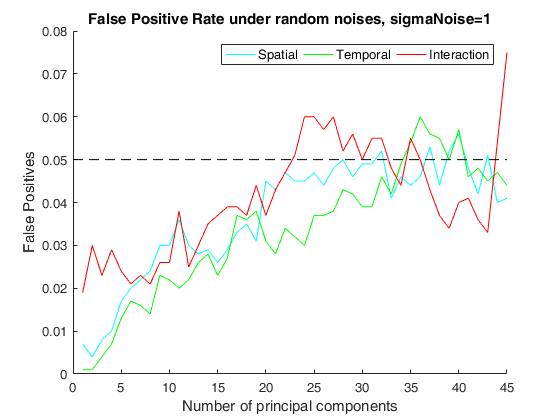
\includegraphics[scale=0.55]{2C__Users_Hao_Dropbox_NewtermPHD_TERM2_SS9833B____of_brain_imaging_data_Report_MANOVA_PCA_Sig.png}}\subfloat{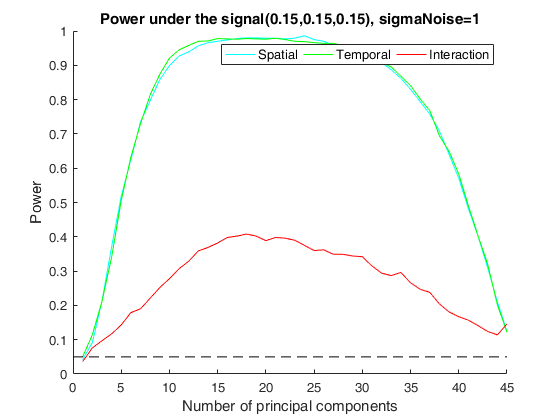
\includegraphics[scale=0.55]{3C__Users_Hao_Dropbox_NewtermPHD_TERM2_SS9833B_____brain_imaging_data_Report_MANOVA_PCA_Power.png}}\protect\caption{{\footnotesize{}CV-MANOVA using the first $N$ principal components
of voxels: The left figure shows the false positive rates for detecting
each term from 1000 simulations of random noises. The right figure
shows the power for detecting each term from 1000 simulations of signals,
with 0.15 scale for each term. Under both cases, the variance for
the random error term is 1. ($N=1,\ldots,45$) }{\small{}\label{fig:CV-MANOVA-PCA}}}
\end{figure}


\begin{figure}[H]
\centering{}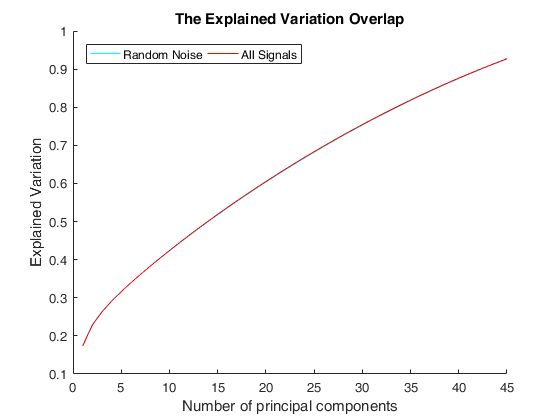
\includegraphics[scale=0.55]{4C__Users_Hao_Dropbox_NewtermPHD_TERM2_SS9833B____in_imaging_data_Report_MANOVA_PCA_Variation.png}\protect\caption{Explained Variance of PCA\label{fig:Explained-Variance-of}}
\end{figure}



\subsection{Power under Different Hypotheses}

To compare the power of different methods under different hypothese,
we did 1000 simulations under different hypothesis and the results
are shown by Figure \ref{fig:MANOVA-ss} to Figure \ref{fig:CVMANOVA-ss}.
The three digits in the legend represents if there is an effect of
the spatial pattern, the temporal pattern or the interaction, where
0 indicates no such patterns and 1 indicates the signal for the pattern
is 0.15. The curves with no markers were set to the null distribution
for performing statistical tests, because the the pattern of interest
did not exist. Hence the numbers besides the curves with markers indicate
the power for detecting the pattern in the corresponding alternative.
We can see that the CV-MANOVA enhanced the powers for both main effects
and interactions. We also found out that the CV-MANOVA was approximately
unbiased when the data is generated from random noises, but there
was a drift for the distribution of the spatial pattern when the interaction
was involved.

\begin{figure}[H]
\begin{centering}
\subfloat{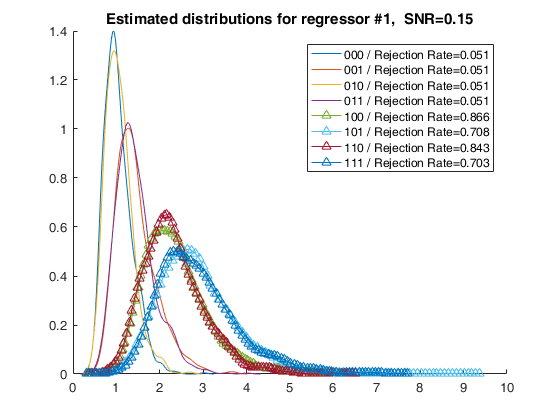
\includegraphics[scale=0.55]{5C__Users_Hao_Dropbox_NewtermPHD_TERM2_SS9833B_____imaging_data_Report_MANOVA_dist_regressor1.png}}\subfloat{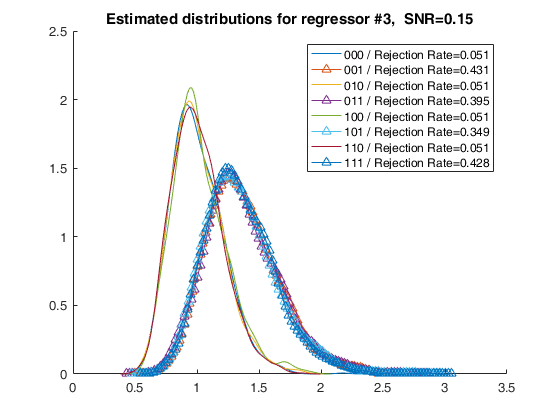
\includegraphics[scale=0.55]{6C__Users_Hao_Dropbox_NewtermPHD_TERM2_SS9833B_____imaging_data_Report_MANOVA_dist_regressor3.png}}
\par\end{centering}

\centering{}\protect\caption{MANOVA using the first $28$ principal components under difference
hypotheses: the left figure shows the power for detecting the spatial
pattern and the right figure is for the interaction.\label{fig:MANOVA-ss}}
\end{figure}


\begin{figure}[H]
\begin{centering}
\subfloat{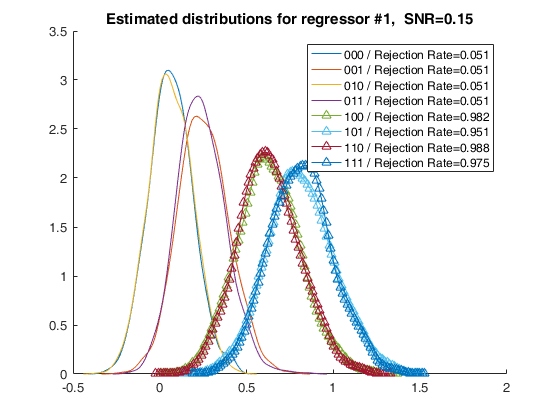
\includegraphics[scale=0.55]{9C__Users_Hao_Dropbox_NewtermPHD_TERM2_SS9833B____maging_data_Report_CVMANOVA_dist_regressor1.png}}\subfloat{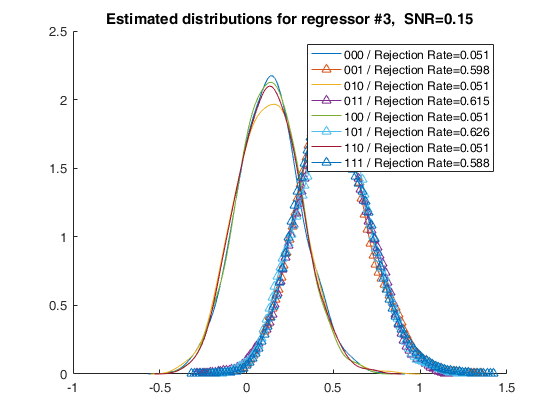
\includegraphics[scale=0.55]{10C__Users_Hao_Dropbox_NewtermPHD_TERM2_SS9833B___maging_data_Report_CVMANOVA_dist_regressor3.png}}
\par\end{centering}

\centering{}\protect\caption{CV-MANOVA under difference hypotheses: the left figure shows the power
for detecting the spatial pattern and the right figure is for the
interaction.\label{fig:CVMANOVA-ss}}
\end{figure}



\subsection{Noise Tolerance of MANOVA and CVMANOVA}

In order to see how the power of each method is related the signal-noise-ratio
(SNR), we did 1000 simulations with four different SNR's. The null
hypothesis for each method was set as random noises. Figure \ref{fig:MANOVA-SNR}
to Figure \ref{fig:CVMANOVA-SNR} show that the power of each method
increased dramatically as the SNR increased.

\begin{figure}[H]
\begin{centering}
\subfloat{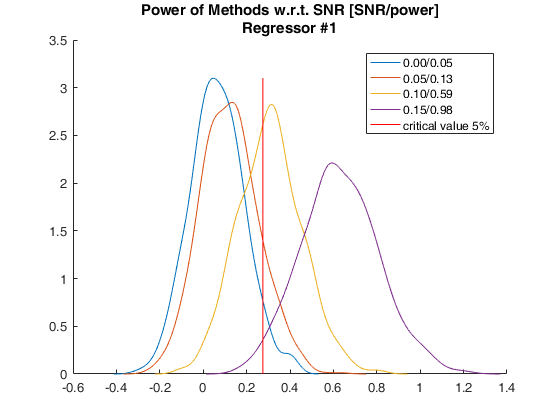
\includegraphics[scale=0.55]{7C__Users_Hao_Dropbox_NewtermPHD_TERM2_SS9833B____imaging_data_Report_MANOVA_power_regressor1.png}}\subfloat{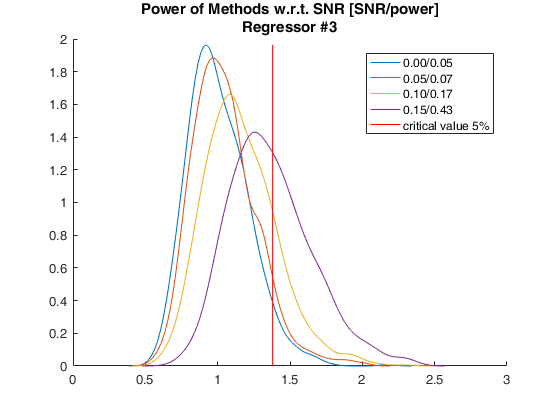
\includegraphics[scale=0.55]{8C__Users_Hao_Dropbox_NewtermPHD_TERM2_SS9833B____imaging_data_Report_MANOVA_power_regressor3.png}}
\par\end{centering}

\centering{}\protect\caption{Power v.s. SNR for MANOVA using the first $28$ principal components
under difference hypotheses.\label{fig:MANOVA-SNR}}
\end{figure}


\begin{figure}[H]
\centering{}\subfloat{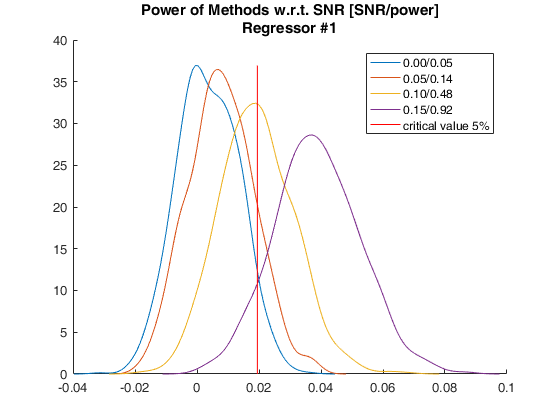
\includegraphics[scale=0.55]{11C__Users_Hao_Dropbox_NewtermPHD_TERM2_SS9833B___aging_data_Report_CVMANOVA_power_regressor1.png}}\subfloat{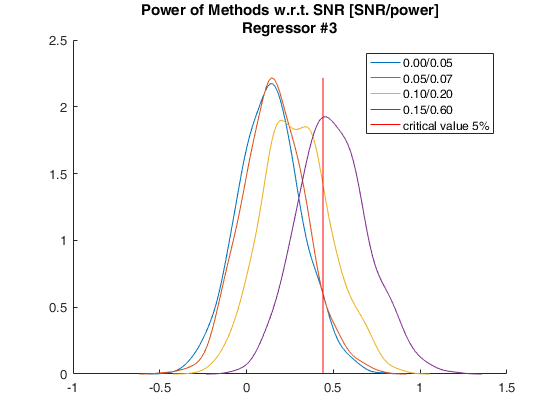
\includegraphics[scale=0.55]{12C__Users_Hao_Dropbox_NewtermPHD_TERM2_SS9833B___aging_data_Report_CVMANOVA_power_regressor3.png}}\protect\caption{Power v.s. SNR for CVMANOVA \label{fig:CVMANOVA-SNR}}
\end{figure}

 

\FloatBarrier

\section{Classification approach}\label{sec:classification}


This section follows the ideas presented in~\cite{Kornysheva2014}. 
Generally, we are to measure the difference in reactions of voxels to different combinations of conditions. 
Machine learning studies different algorithms that are able to find regularities within object's features in order to extract some information about the object. In particular, classification problem is to train a classifier, a function that maps features of the object to the class that this object belongs to. 

\subsection{K-Nearest-Neighbors (KNN) classifier}

\begin{figure}[ht]
\centering
\begin{minipage}[c]{0.3\textwidth}
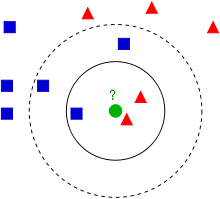
\includegraphics[width=0.9\textwidth]{220px-KnnClassification.png}
\end{minipage}
\begin{minipage}[c]{0.6\textwidth}
\caption{Example of KNN classification. The test sample (green circle) should be classified either to the first class of blue squares or to the second class of red triangles. If K = 3 (solid line circle) it is assigned to the second class because there are 2 triangles and only 1 square inside the inner circle. If K = 5 (dashed line circle) it is assigned to the first class (3 squares vs. 2 triangles inside the outer circle). Credit to https://en.wikipedia.org/wiki/K-nearest\_neighbors\_algorithm\#/media/File:KnnClassification.svg}
\label{fig:knn_example}
\end{minipage}
\end{figure}

One of the simple classifiers is \emph{ K-Nearest-Neighbors} (KNN) classifier, see \autoref{fig:knn_example}.
Given feature vector $x$ and training set $Tr=(\{x_i\},\{c_i\})$ a classical KNN classifier predicts classification label $c$ such that 
$$c^*(x)\;\; := \;\; \arg\max_y \#\{i : x_i \in knn(Tr,x) \;\&\; c_i=y \}$$ where $knn(Tr,x)$ is the set of $K$ nearest neighbors of vector $x$ from the set $\{x_i\}$. The classifier can be used to produce a confidence measure $conf(x,c,Tr)$ that shows the likelihood of test vector $x$ belonging to class $c$:
 $$ conf(x,c,Tr) \;\; := \;\; \frac{\#\{i : x_i \in knn(Tr,x) \;\&\; c_i=y \}}{K}. $$ The value of $conf(x,c,Tr)$ reaches its maximum value of $1$ if all K nearest neighbors are from class $c$. %$conf(x,c)$ generates a soft score of class $c$ given feature vector $x$.

Given test dataset $R=(\{x'_i\},\{c'_i\})$ where $\{x'_i\}$ are feature vectors and $\{c'_i\}$ are true class labels, we define the average accuracy (AC) of classification as 
\begin{equation}
AC(R,Tr) \;\; := \;\; \frac1{|R|}\sum_i conf(x'_i, c'_i,Tr).
\label{eq:ac}
\end{equation}
Note that $AC(R,Tr)$ is an estimator of the probability of correct classification. If accuracy is close to 1 the classifier is able to distinguish feature vectors coming from different classes. That means that features~$x_i$ contain a lot of information about classes $c_i$ they originate from. On the other hand, if features~$x_i$ do not contain relevant information about class $c_i$ the classifier will not be able to predict correct class better than random guessing\footnote{It is in case of balanced data, i.e. the number of representatives of different classes is the same in the training set.}. In this case the accuracy will be $\frac1{|C|}$ where $|C|$ is the number of different classes. 

\subsection{Cross-validation}

\newcommand{\CVAC}{CV\!\!AC}

Cross-validation is a powerful technique that allows to estimate unbiased statistics, e.g. the average accuracy, in situations where the test data is not provided. Suppose that given training set $Tr$ is partitioned into $n$ folds $Tr=\cup_{i=1}^n T_i,$ then \emph{cross-validated average accuracy} is $$\CVAC(Tr) \;\; := \;\; \frac1n\sum_{i=1}^n AC(T_i,Tr \setminus T_i).$$ If the training set is partitioned in a way that folds are independent on each other $\CVAC(Tr)$ is an unbiased estimator of the probability of correct classification.

\begin{figure}[t]\centering
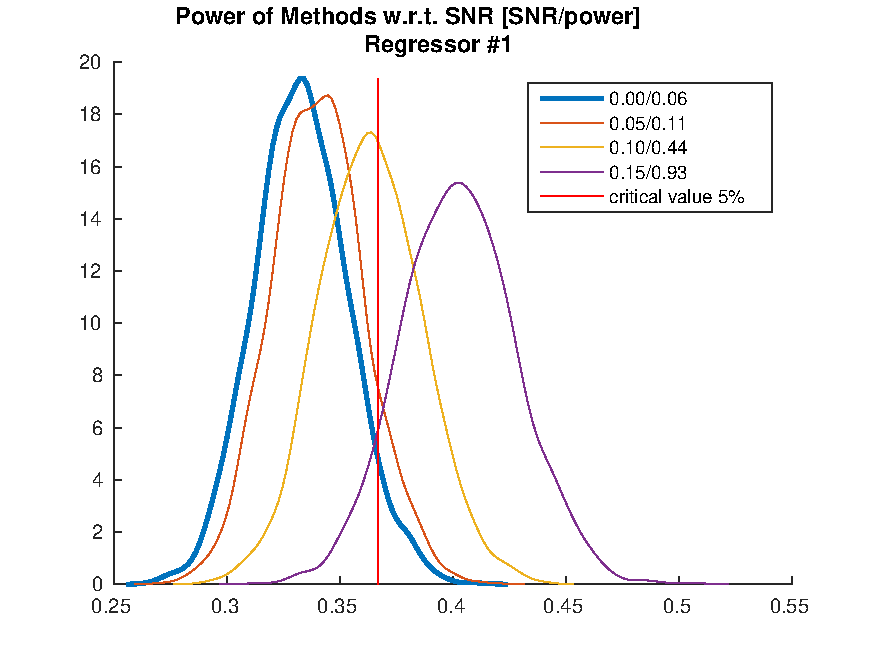
\includegraphics{sample_knn_conv_1}  
\caption{KNN: Estimated distribution (probability densities) of the average accuracy of KNN classifier w.r.t different levels of signal noise ratio (SNR). We test the presence of the main effect against pure noise (bold blue curve). The critical value (red vertical bar) is chosen as $95$ percentile of H0 distribution (bold blue curve). The power is the rate of rejection of H0 in the presence of the main effect. The legend on the plot shows the SNR and power of the statistic test. The power reaches level of $93\%$ at SNR=$0.15$.}\label{fig:knn convergence}
\end{figure}

\subsection{Factorial pattern analysis of fMRI data}

In factorial pattern analysis of fMRI data we are interested in the following question. Does a given region of the brain (represented as activation pattern of voxels) encode information about different conditions and their interaction? One way to answer this question is to train a classifier that predicts the condition that resulted in the observed activation pattern. If the classifier predicts the correct condition significantly better than random guessing then the answer to the question is positive.

In our experimental setting there are 2 factors (T and S), each of them has 3 levels. Each test run measures 9 (one for each combination of factors) activation pattern in 160 voxels. The total number of runs is 6. This yields 54 feature vectors of dimensionality 160. Each run naturally forms an independent fold for cross-validation.

\subsection{Main effect detection}

In this subsection we are interested in detecting the presence of the main effect of a factor. Activation patterns measured under different levels of the factor are significantly different from each other, if the main effect is present. This, in principle, allows a classifier to distinguish the patterns. So, to detect the main effect we train our KNN classifier to predict 3 levels of the factor based on activation patterns. We choose $K=10$ as the one that gives the best performance. \autoref{fig:knn convergence} shows the result of the experiment.

\begin{figure}[t]
\begin{tabular}{cc}
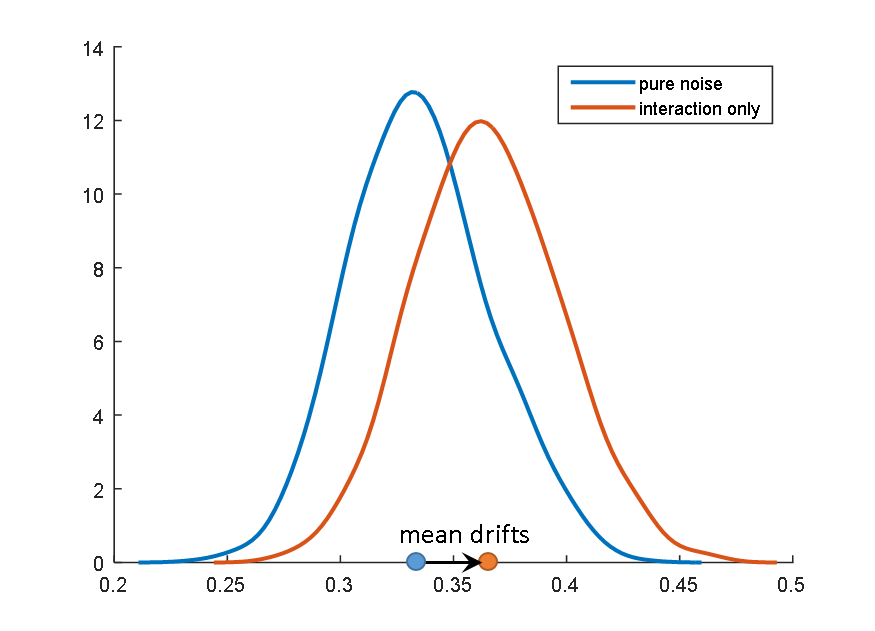
\includegraphics[width=0.5\textwidth]{drift} &
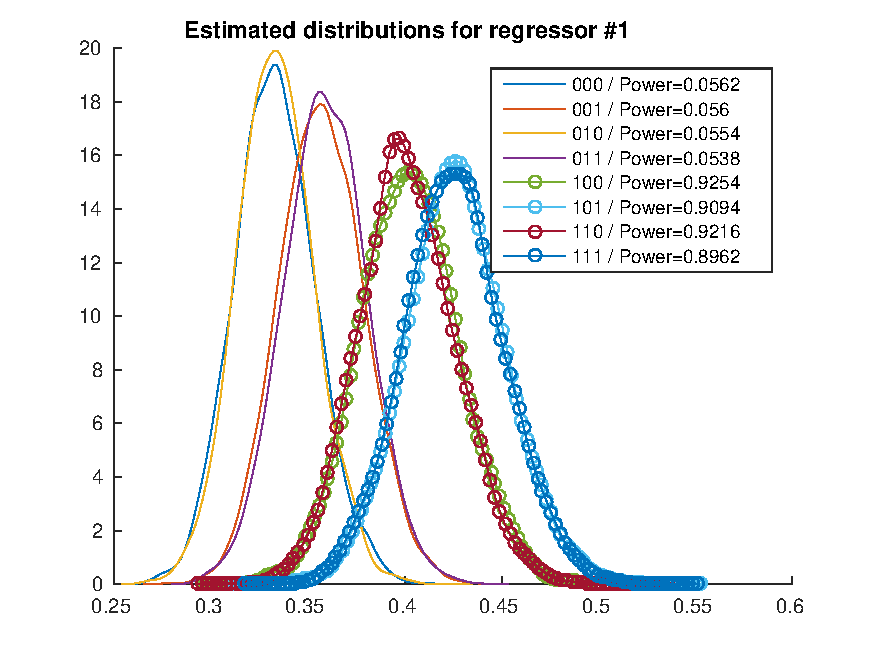
\includegraphics[width=0.5\textwidth]{sample_knn_distributions_1}  \\
(a) & (b) 
\end{tabular}
%\vspace{-6mm}
\caption{KNN: Testing main effect (circle markers) against all possible combinations of other effects (without markers). \newline
{\bf (a)} Note that as soon as some interaction is introduced the expected value of the classification accuracy increases. This is because interaction allows to discriminate different conditions even if no main effect present.\newline
 {\bf (b)} The distribution of the statistic is not invariant to presence of other effects. 0/1 in the legend codes absence/presence of two main effects and interaction between them. Critical value is given by 95\% percentile of H0 distribution. The power is computed as portion of points generated from H1 distribution that are above the critical value.  For example, ``101 / Power = 0.852'' corresponds to H1 s.t. there is no main effect S but there are main effect T and interaction between S and T. H0 in this case is ``001'', i.e. only interaction is present.}\label{fig:knn drift}
\end{figure}

We observe that as we increase the level of interaction the expected cross-validated average accuracy also increases, see \autoref{fig:knn drift}a. The presence of interaction between factors T and S means that there is a unique structure of activation patters that allows distinguishing all 9 possible combinations of the factors significantly better than random guessing. But the ability to decode 9 combinations implies the ability to decode each of the factors. This results in the drift in the average accuracy.

\begin{figure}[t]
\centering
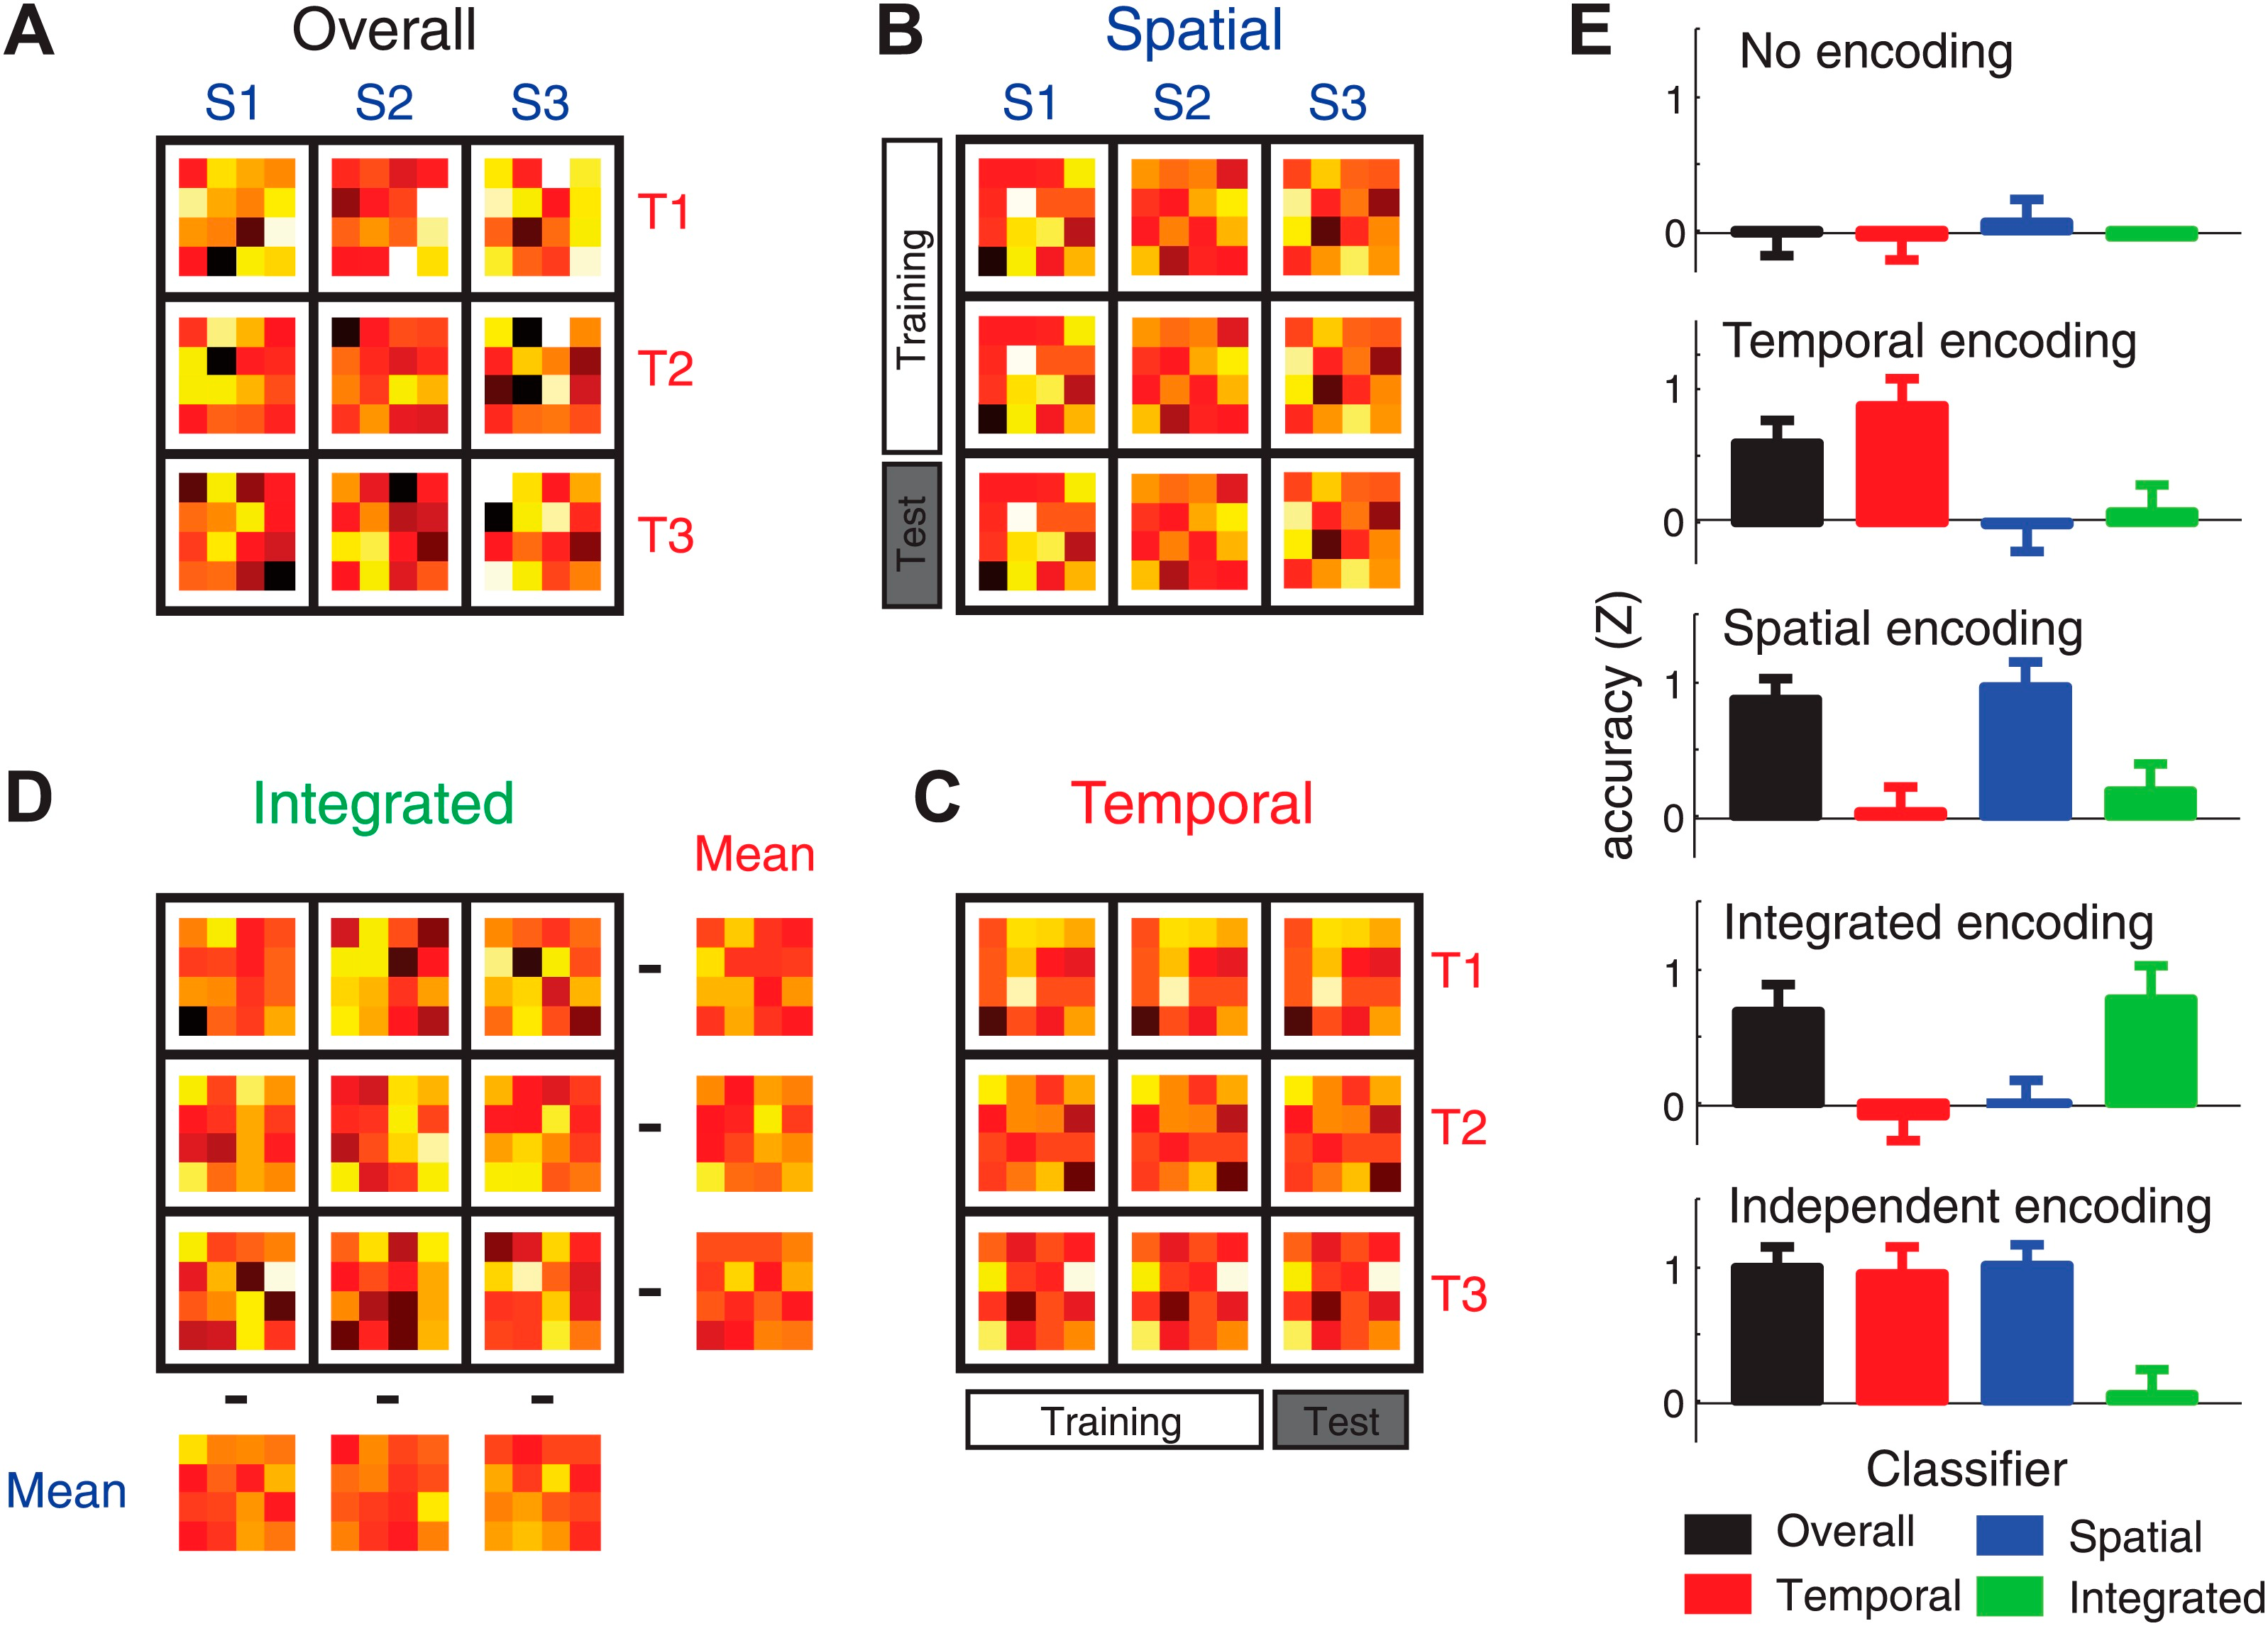
\includegraphics[width=0.60\textwidth,clip=true,trim=0 0 28cm 0]{elife-03043-fig3-v1}
\caption{Two factors have 3 levels: S1,S2,S3 and T1,T2,T3. All possible combination of levels result in 9 measured activation patterns ({\bf A}). Double cross-validation allows to decode the main effects ({\bf B} and {\bf C}) independently from interaction. Mean subtraction for both factors allows to destroy their main effects and detect only interaction ({\bf D}). The plot is by~\cite{Kornysheva2014}}\label{fig:patterns}
\end{figure}

\begin{figure}[p]
\centering
\begin{minipage}[c]{0.5\textwidth}
\centering
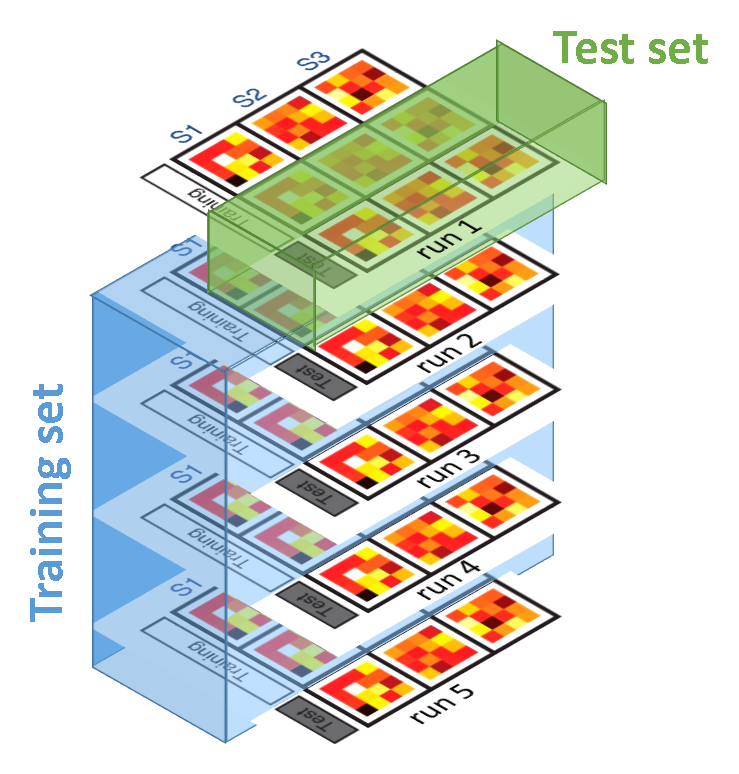
\includegraphics[width=.7\textwidth]{2xval.png}
\end{minipage}\hfill
\begin{minipage}[c]{0.5\textwidth}
\caption{Double cross validation for detecting the main effect of the spatial factor. Suppose one tests a classifier on  patterns that have the temporal factor level of Tn (marked by word test on the plot) and originate from run $i$ (green box on the plot). Then the classifier should be trained on the rest of the patterns except the patterns with the same temporal level Tn or from run $i$ (blue box on the plot).}\label{fig:2xval}
\end{minipage}
\end{figure}

To overcome this issue \cite{Kornysheva2014} propose to use \emph{double cross validation}. See \autoref{fig:patterns}B. Suppose the patterns only contain interaction and there is no main effects. Let's consider the patterns where factor T has the level of Tn. There are three patterns, see lower row in  \autoref{fig:patterns}B. There is a unique structure within this patterns that allows distinguishing between them. How ever the classifier will be able to recognize this structure only if training set contains such combinations of the factors. So, when we test the patterns from factor Tn  we should exclude from the training set the patterns coming from Tn as well, see \autoref{fig:2xval}. This prevents classifier from learning interaction structure while preserves the main effect information, see \autoref{fig:2xval for main effect}.

\begin{figure}[p]
%\begin{subfigure}[t]{0.49\textwidth}
\subfloat[][Testing the main effect for the first factor (circle markers) against all possible combinations (without markers) with double cross-validation. The distributions only depend on the presence of the main effect. Note, there is no drift as in \autoref{fig:knn drift}.]{
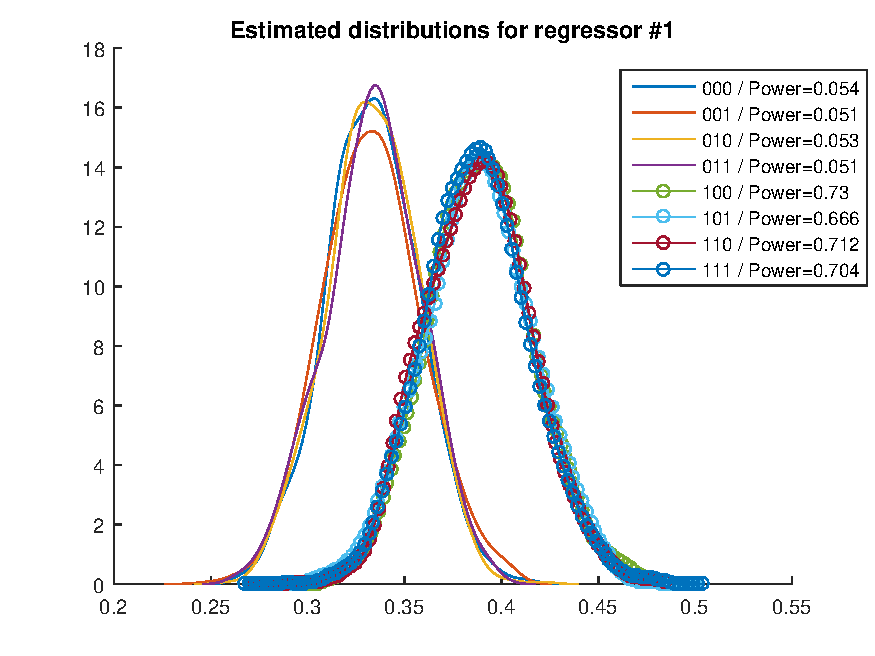
\includegraphics[width=.48\textwidth,clip=true,trim=0 0 0 7.5mm]{sample_knn2_distributions_1}
%\caption{Testing the main effect for the first factor (circle markers) against all possible combinations (without markers) with double cross-validation. The distributions only depend on the presence of the main effect. Note that there is no drift as in \autoref{fig:knn drift}.} 
\label{fig:2xval for main effect}
%\end{subfigure}
}
\hfill
%\begin{subfigure}[t]{0.49\textwidth}
\subfloat[][Testing interaction (circle markers) against all possible combinations (without markers). The distributions only depend on the presence of the interaction.]{
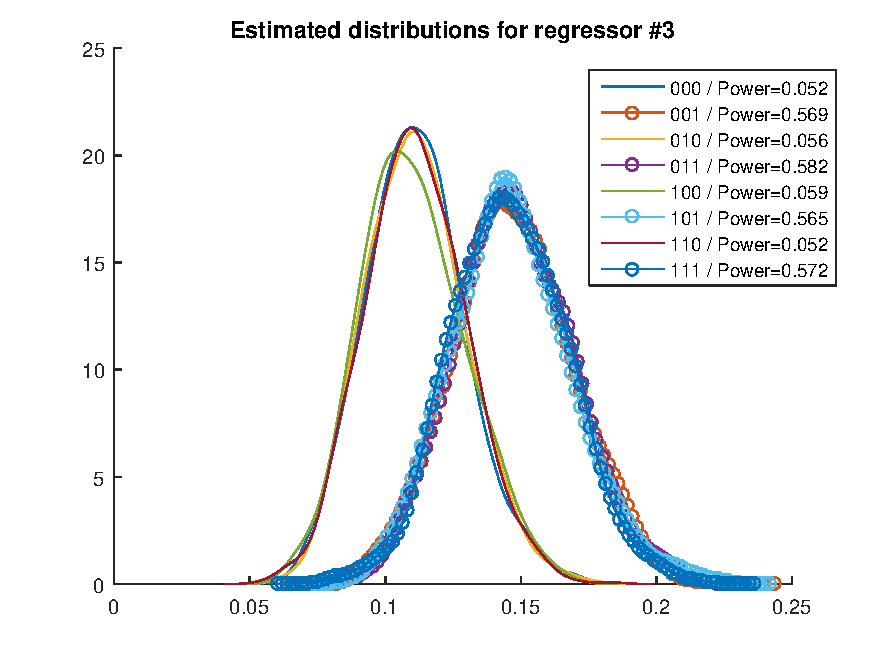
\includegraphics[width=.48\textwidth,clip=true,trim=0 0 0 7.5mm]{sample_knn2_distributions_3}
%\caption{Testing interaction (circle markers) against all possible combinations (without markers). The distributions only depend on the presence of the interaction.} 
\label{fig:test interaction}
}
%\end{subfigure}
\caption{Detection of main effects (a) and interaction (b). Estimated distributions of statistic \eqref{eq:ac} are shown. The legend is described in \autoref{fig:knn drift}. The power is worse than in \autoref{fig:knn convergence} due to smaller training set.}
\end{figure}


\subsection{Interaction detection}

To detect interaction  we train a classifier to decode all 9 possible combinations of factor levels. However, if there is no interaction but only main effects the classifier will be able to recognize 9 classes with chances significantly higher than random guessing. \cite{Kornysheva2014} propose to subtract the mean pattern computed withing each factor level, see \autoref{fig:patterns}D. Indeed, the main effect of a fixed factor level is constant and remains the same in the mean pattern. If we subtract the mean pattern we remove main effect from the patterns, see \autoref{fig:test interaction}.

\subsection{Results and conclusions}

\begin{figure}[p]
\subfloat[][Main effect detection with double cross-validation. The power converges to 1 as SNR increases.]{
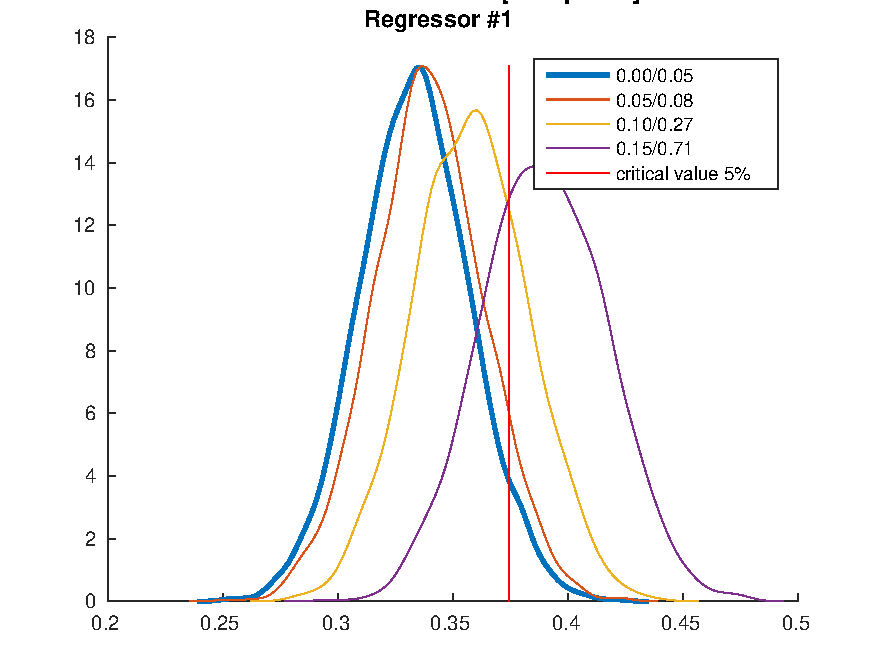
\includegraphics[width=.48\textwidth,clip=true,trim=0 0 0 8mm]{sample_knn2_conv_1}
\label{fig:knn2 convergence:main}
}
\hfill
\subfloat[][Interaction detection with mean subtraction.]{
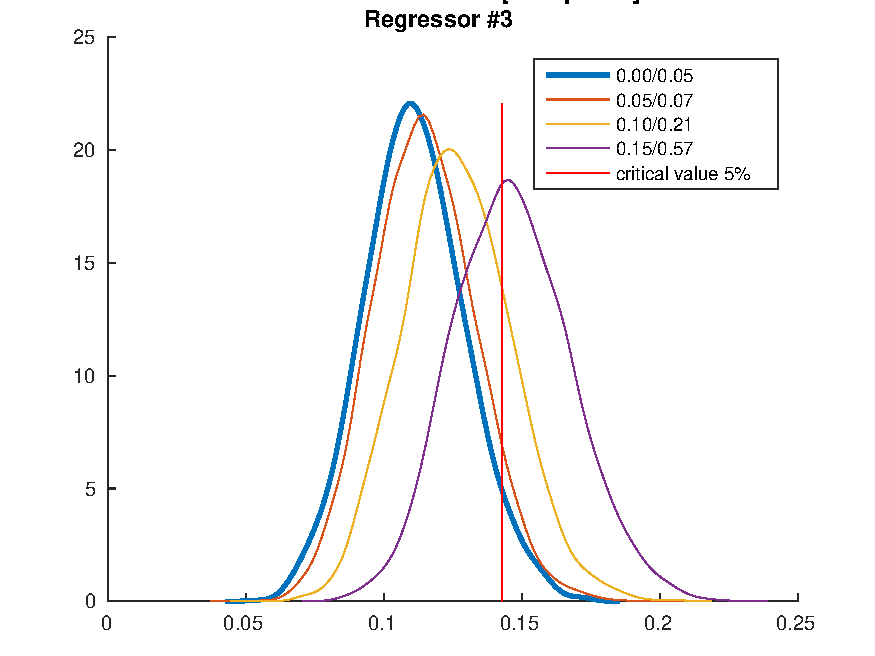
\includegraphics[width=.48\textwidth,clip=true,trim=0 0 0 8mm]{sample_knn2_conv_3}
\label{fig:knn2 convergence:int}
}
\caption{Main effect and interaction detection. Estimated distributions of average accuracy \eqref{eq:ac} are shown. The power rapidly increases as Signal-to-Noise-Ratio (SNR) increases.}
\label{fig:knn2 convergence}
\end{figure}

The classification approach is a very powerful technique for decoding the activation patterns. It relies on a very popular and established field of machine learning that allows removing the limitations on the number of voxels and assumption of normality of the data. Our experiments show that the approach allows reliable detection of the main effects and interaction. With SNR level of 0.15 the power of the proposed statistical test (base on average accuracy) reaches the level of $\sim71\%$ for main effect detection (\autoref{fig:knn2 convergence:main}) and $\sim57\%$ for interaction (\autoref{fig:knn2 convergence:int}). We also show that as SNR increases the power of our statistical test reaches 1 very quickly (\autoref{fig:knn convergence}). We also show that the proposed statistic~\eqref{eq:ac} coupled with double cross-validation for main effect and mean subtraction for interaction detection is always unbiased in all combinations of factors, see \cref{fig:2xval for main effect,fig:test interaction}.


\section{Pattern component modeling}\label{sec:pcm}

\input{harrison.tex}

\FloatBarrier

\section{Discussion}\label{sec:discussion}

\begin{figure}[ht]
\centering
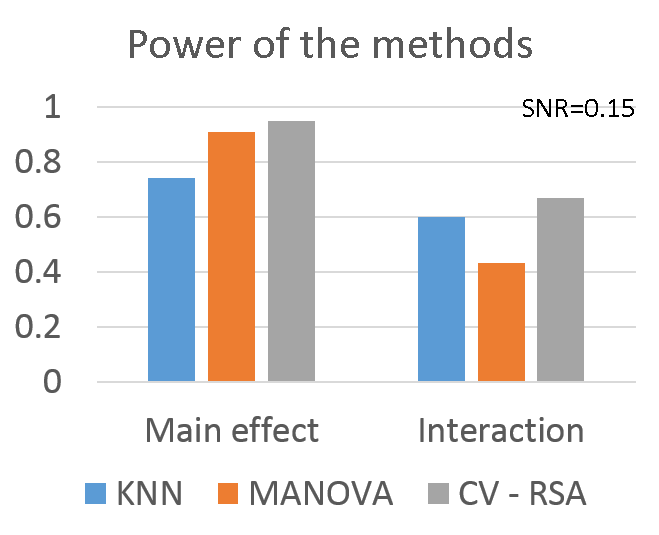
\includegraphics[width=0.5\textwidth]{overall.png}
\caption{Comparison of different methods. Pattern component modeling (PCM) performs the best.}
\label{fig:overall}
\end{figure}

In this project we implemented and evaluated three different methods. Those are Multivariate Analysis of Variation (MANOVA), Classification approach and Pattern component modeling (PCM). The comparison is summarized in \autoref{fig:overall}. In our simulation experiments we found that classical MANOVA limitations on the number of voxels can be compensated by PCA dimensionality reduction. The resulting PCA-MANOVA method gives competitive results for main effect detection. Quite general classification approach yields slightly lower power for the main effect detection and outperforms PCA-MANOVA in case of interaction detection. We found out that PCM performs the best among all competitive methods.

However, there are some limitations of our research. Our simulation procedure assumes normal uncorrelated distribution of activation patterns. Both assumptions (normality and uncorrelatedness) are ideal and hard to achieve in practice. Our implementation of MANOVA and PCM significantly rely on this assumptions. The classification approach does not rely on this assumption. In our work we only evaluated one classifier, namely K Nearest Neighbor classifier. Other, more powerful classifiers might yield better results.

\FloatBarrier

\bibliographystyle{unsrt}
\bibliography{ref,../CliffordReport/ref,../HarrisonMethod/ref}

\end{document}
